\begin{frame}{Information Preserving Refinement (IPR)}
  \begin{columns}
  \column{0.48\linewidth}
  \begin{outline}
    \1 Start with functional specification 
    \1 Device implements this spec
    \1 Wire-level interactions $\iff$ spec. level operations 
    \1 Implementation States $\iff$ spec. level states
    \1 Based on dual view
    \2 Real world (uncompromised host)
    \2 Ideal world (compromised host
  \end{outline}

  \column{0.48\linewidth}
  \centering
  \begin{center}
    \shadowimage[width=3.5cm]{func_spec.png}
  
    \vspace{0.5cm}

    
    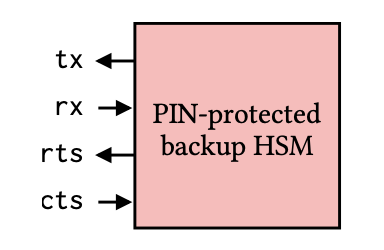
\includegraphics[width=3cm]{wire_diagram.png}
  \end{center}
\end{columns}
\end{frame}

\begin{frame}{Information Preserving Refinement (IPR)}
  \centering
  \begin{center}
    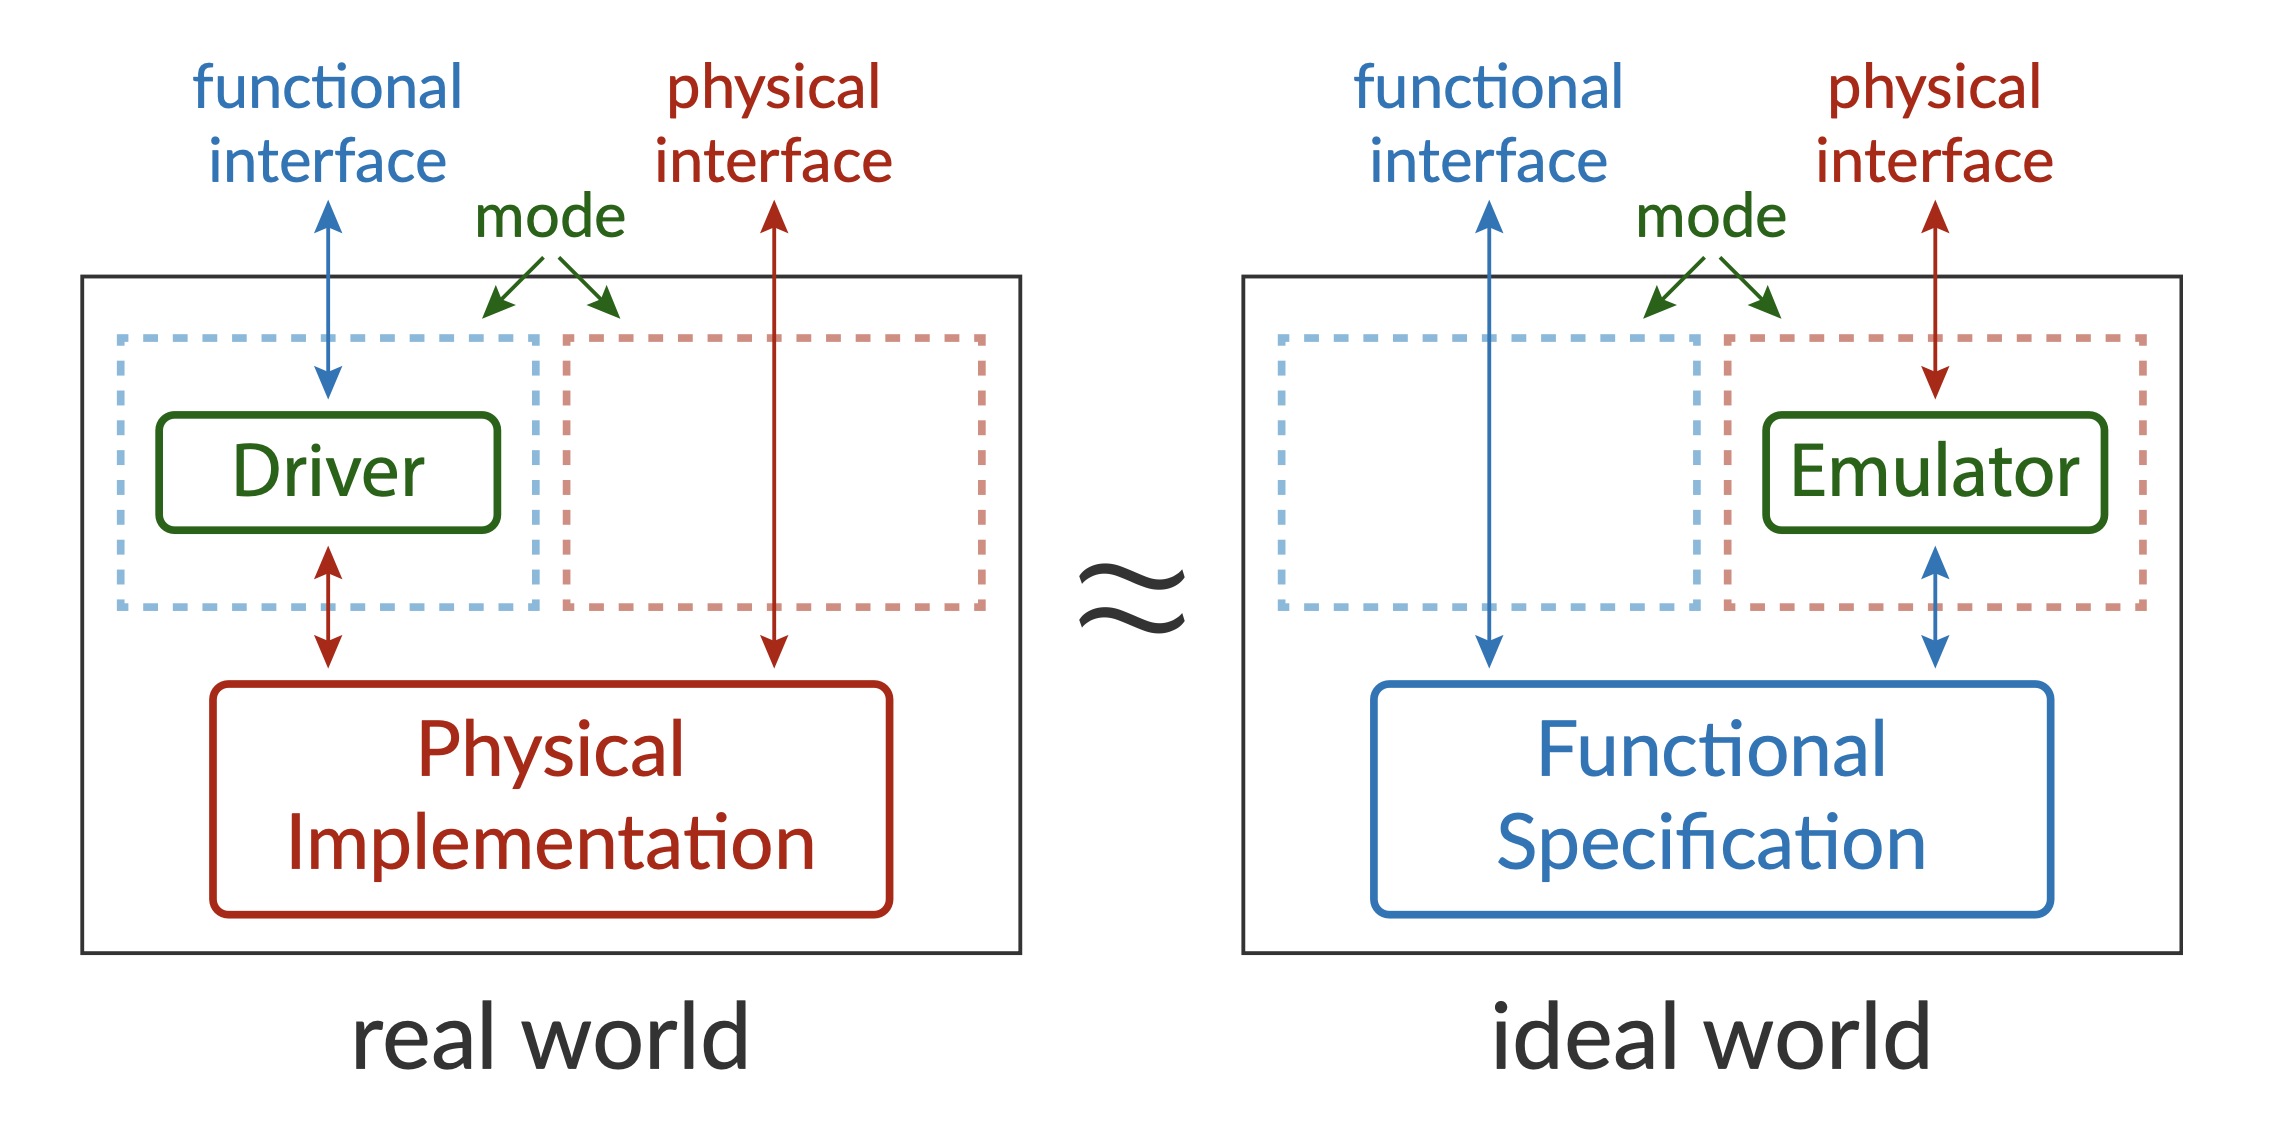
\includegraphics[width=11cm]{ipr.png}
  \end{center}

\end{frame}

\placelogofalse
\begin{frame}{Proving IPR}
  \begin{columns}
  \column{0.48\linewidth}
  \begin{outline}
    \1 Developer provides $R$, relates
    \2 State of spec state machine
    \2 State of implementation
    \1 Developer also provides
    \2 Driver
    \2 Emulator
  \end{outline}

  \column{0.48\linewidth}
  \begin{center}
    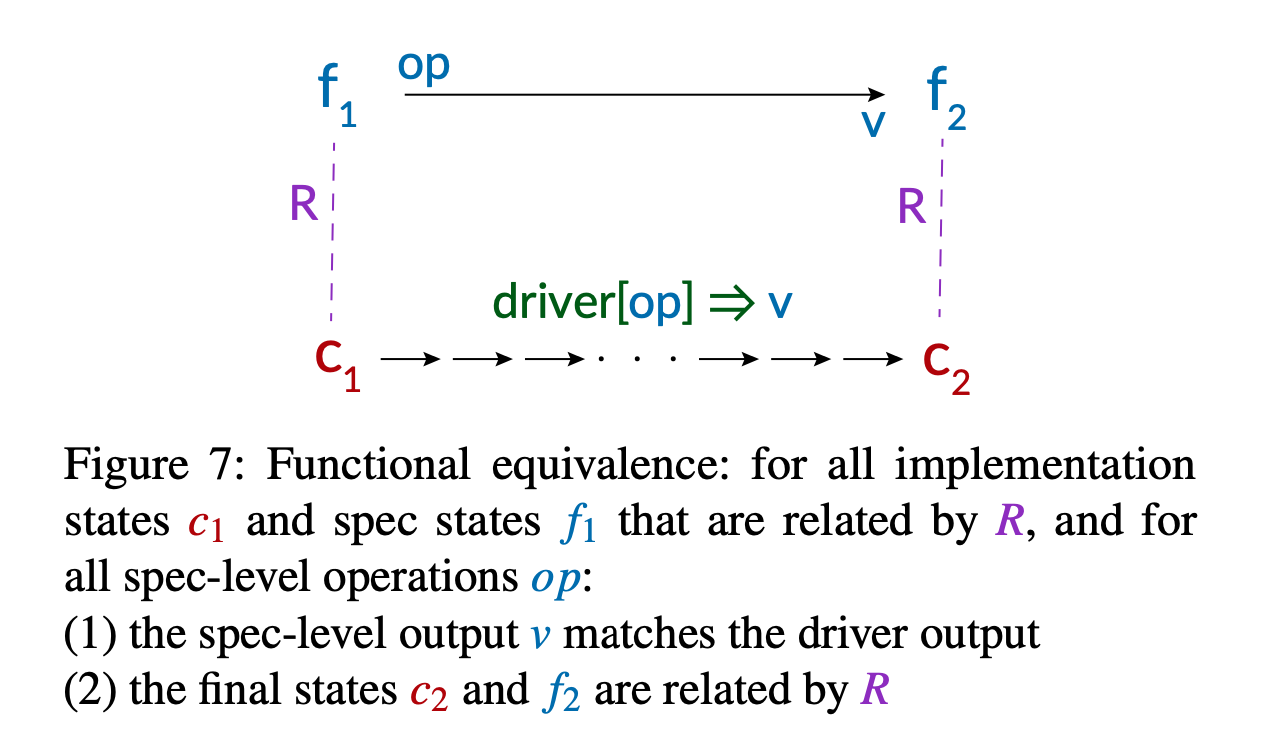
\includegraphics[width=4.5cm]{fig_7.png}

    \vspace{0.5cm}

    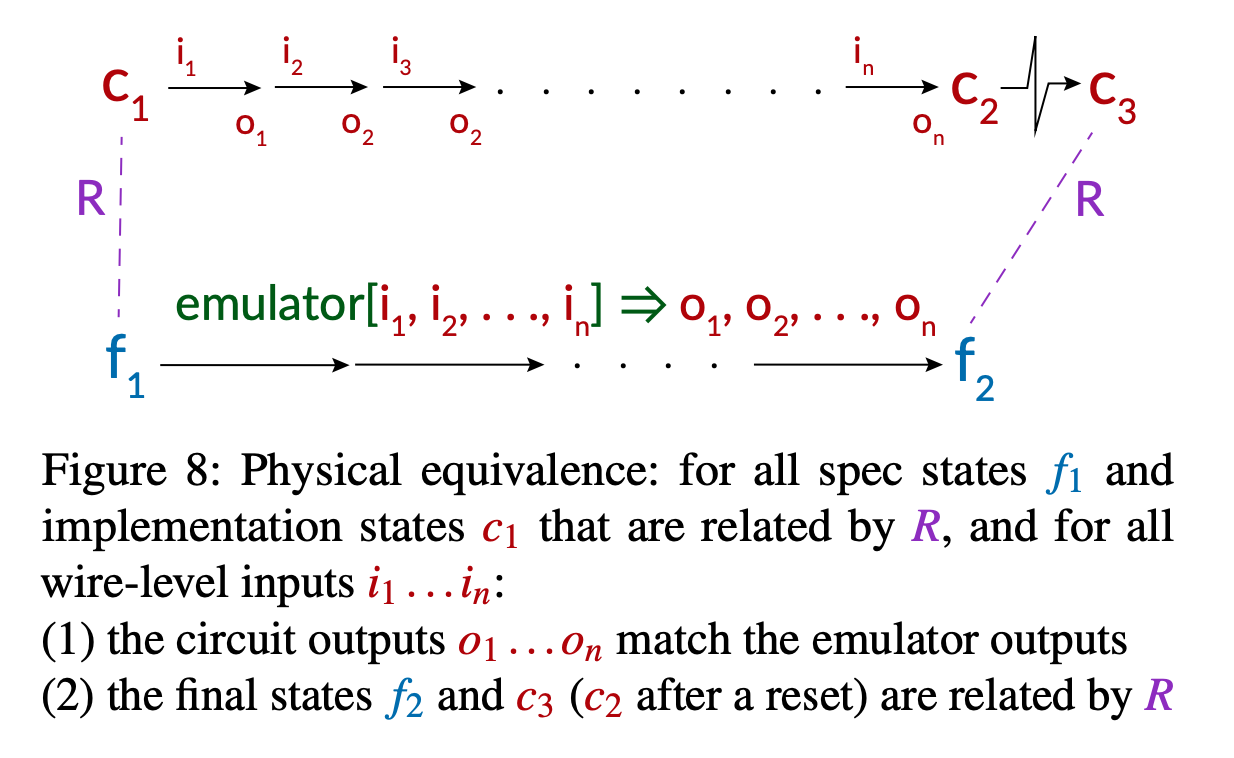
\includegraphics[width=4.5cm]{fig_8.png}

  \end{center}
  \end{columns}
\end{frame}
\placelogotrue
